\documentclass[12pt,twoside]{reedthesis}
\usepackage{graphicx,latexsym} 
\usepackage{amssymb,amsthm,amsmath}
\usepackage{longtable,booktabs,setspace} 
\usepackage{url}
\usepackage{natbib}
\usepackage{algorithm}
\usepackage{algorithmic}

\title{My Final College Paper}
\author{Ivan A. Malison}
\date{April 2012}
\division{Mathematics and Natural Sciences}
\advisor{James D. Fix}

\department{Mathematics}


\setlength{\parskip}{0pt}
\begin{document}

  \maketitle
  \frontmatter 
  \pagestyle{empty}

  \chapter*{Acknowledgements}

% The preface is optional
% To remove it, comment it out or delete it.
    \chapter*{Preface}

    \tableofcontents

    \chapter*{Abstract}
	
	\chapter*{Dedication}

  \mainmatter 
  \pagestyle{fancyplain}

    \chapter*{Introduction}
         \addcontentsline{toc}{chapter}{Introduction}
	\chaptermark{Introduction}
	\markboth{Introduction}{Introduction}

A graphics processing unit, or GPU, is a component of a digital computer is most accurately described as a computer on a chip. In the past decade, graphics card architecture has undergone a slew of revolutionary changes that have transformed GPUs from highly specialized graphics processors, to massively parallel high-end computers.

GPUs render images into a special type of memory called a frame buffer through a complicated multi-stage process called the graphics pipeline. Though GPUs have existed in some form or another since the early 1980s, the architecture of the modern GPU has bears resemblence to those of its early predecessors.

Until the early 2000s, GPUs were fixed-function graphics pipelines. That is to say that each stage of the graphics pipeline was performed by a distinct piece of circuitry that was explicitly designed to handle that task. Application Developers configured the operation of these GPUs through APIs like Microsoft's Direct X and its non-proprietary equivalent OpenGL, but none of the pipeline stages were truly programmable.

This began to change in 2001, when the major GPU vendor NVIDIA released the GeForce 3. This graphics card allowed application developers to directly program one of the stages of the graphics pipeline. Eventually, other stages of the graphics pipeline were also opened to application developers.

By the mid to late 2000s GPUs had begun had begun to resemble massively parallel computers. Though GPUs still contained significant amounts of fixed function circuitry, the various programmable stages of the graphics pipeline were now being performed by a single multi-function array of processors. At this point, some objective measures of performance placed consumer grade GPUs ahead of the best CPUs of the same era. The raw computational performance available in GPUs enticed some researchers to attempt to perform non-graphical computations on GPUs. Though the GPU APIs available during this time period were far more flexible than those of previous eras, they were still ultimately aimed at rendering graphics. Many of the stages of the graphics pipeline remained fixed function, and all output generated by the GPU was still written into a fixed location called the frame buffer. Despite these drastic limitations, some researchers were able to acheive promising results by cleverly mapping non-graphical calculations into ones that could be performed by a GPU.

This movement culminated led NVIDIA to develop the CUDA C/C++ software package.





\chapter{GPU Hardware}
Though the architecture of modern GPUs can be characterized in general ways, there is actually a great deal of diversity in the circuity and operation procedures of different graphics cards, even between those that are produced by the same vendor. The CUDA and OpenCL APIs allow Application Developers write code that can be compiled to run efficiently on nearly any modern GPU, without knowing the details of every GPU on the market. In fact, it is entirely possible to write functioning CUDA or OpenCL code with almost no knowledge of modern GPU architecture. However, to write programs that perform optimally, it is absolutely essential to have a rudimentary understanding of the basic features of modern graphics hardware.

The following chapter describes the basic design of modern GPUs. Though the architectural features highlighted in this section will inform the development of algorithms developed later in the paper, keep in mind that this description is a something of a cartoon, and that actual GPU hardware is usually more sophisticated.

\section{The Graphics Pipeline}

To this day, GPUs are devices that are primarily targeted at rendering graphics. Nearly every development in the evolution of graphics hardware has been guided by the goal of making graphics computations faster. As such, it is imparative to understand the basic operation of the graphics pipeline before delving deeper into the hardware features of GPUs.

Though the details of the graphics pipeline are constantly changing and evolving, the fundamental processes involved in the procedure have remained the same for quite some time. What follows is a rough outline of the major steps in the graphics pipeline.

\subsection{Overview of the Graphics Pipeline}

%%insert figure%%

The input to the graphics pipeline consists of an array of polygons, usually triangles, that are positioned in a three dimensional coordinate system. The ultimate goal of the graphics pipeline is to take this data, together with lighting and texture data, and transform it into a 2D image that can be displayed on a screen.

The process begins with a per vertex operation stage, where basic operations are applied to each vertex that makes up one of the triangles in the input array. The vertices are shaded according to their interactions with light in the scene, and sometimes they are rotated and translated. Then the vertices are mapped on to screen space according to some point of view that is often called the virtual camera'.  At this point the vertices are often reassembled, and vertices that will not appear in the final image are discarded.

The next major stage is the rastorization phase. This phase calculates which pixels in the final image will be covered by each primitive from the previous phase. Each primitive generates what is called a fragment at every pixel location that it covers. In the rest of the graphics pipeline, operations take place on a per fragment basis. Note that there is not necessarily a one-to-one association between fragments and pixels because it is possible for multiple primitives to cover the same pixel.

The fragment stage computes a final color value for each fragment generated in the rasotrization phase. This is done by combining color information from vertices, lighting information, and sometimes fetching data from images called textures from device memory.

The final stage computes the final color value for each pixel, usually by selecting the fragment value that is closest to the camera.

\subsection{The GPU Approach}

The distinguishing feature of the graphics pipeline is its enourmous potential for parallelism. Within each stage, the operations that are performed on the primitives that make up the input data, and later, the fragments that are generated from those primitives are all completely independent of one another. Furthermore, operations can be performed on primitives that have reached one stage of the graphics pipeline even if not all of the primitives have yet reached that stage of the pipeline.

If one were to implement the graphics pipeline on a sequential computer they would be forced to start at some stage with some element (or group of elements), and walk through the entire graphics pipeline with that element and its descendants. Then the CPU would move on to the next group of elements, again performing operation on each of the elements. The CPU divides the graphics pipeline in time; at any given moment, it is devoting all its resources to performing the operations at a particular stage for a particular element.

The GPU takes a wildly different approach in which it divides its resources amongst the different stages of the graphics pipeline. This approach to the problem proved to be highly successful for a variety of reasons. The most important of these is that dividing the problem in this manner allowed the hardware that was working in each stage to exploit the data parallelism at that stage. Instead of operating on a single element at a time, a component in the graphics pipeline works on a huge number of objects at a time. Though a graphics component may take quite a long time to compute the desired values for any particular element, it compensates for this by having enourmous throughput. Because the different stages of the graphics pipeline exhibit parallelism over different kinds of primitives, this would not be possible if GPUs attacked the pipeline as a whole. Since each primitive element undergoes the same set of operations, albeit with a different data values, at each stage, this parallelism is accomplished without complicated control circuitry governing the execution on each element.

\subsection{The evolution of GPU Architecture}

Another reason for the initial success of the GPU approach was that many of the computations in the graphics pipeline could be performed more efficiently with specialized hardware. The early graphics hardware architecture, now generally referred to as the fixed-function graphics pipeline, used specialized non-programmable circuitry for each stage in the graphics pipeline. But this design paradigm was not without its downsides. For example, while programmers could control things like the position and intensity of lighting sources through the graphics APIs that controlled these early GPUs, they could not control the algorithm that computed the interactions of those lighting sources with vertices and primitives.

This meant hardware vendors had to add entirely new circuitry to implement any new features that developers requested. For certain kinds of complex lighting and shading effects, it was entirely unfeasible to design circuitry with only those functions in mind. This led graphics hardware vendors to design GPUs where the per vertex operations of the graphics pipeline were performed by hardware that could be directly programmed by application developers. This evolution in graphics hardware proved to be very successful, and eventually, the per fragment and geometry stages of the graphics pipeline became programmable.

Initially, the various programmable stages of the graphics pipeline featured different instruction sets that were suited to the roles they performed. But as the per vertex and per fragment programs that developers were building became increasingly complex, the needs at each stage converged. This led graphics hardware vendors to develop the unified shader model, an architecture paradigm where all of the programmable stages of the graphics pipeline are performed on a single array of multiprocessors. This revolution in graphics card architecture was important for two major reasons. The first of these was that it allowed GPUs to load balance the stages of the graphics pipeline. A fixed-function graphics pipeline was only as fast as its slowest component, because if one stage of the graphics pipeline required more time than the others, all of the other components would become inactive while the slower component finished its computation. With the unified shader model, the resources of the graphics card could be dynmically allocated between the various programmable stages of the graphics pipeline, and most of the hardware would remain active throughout the entire computation.

The other major advantage of this architectural change has nothing to do with the graphics pipeline. With the unified shader model, the instruction sets of the multiprocessor arrays of GPUs have come to resemble those of general purpose processors quite closely. This combined with the release of APIs like CUDA and OpenCL that allow programmers to bypass the graphics pipeline and directly access the multiprocessor arrays of GPUs has greatly facilitated the practice of GPU computing.

\section{The Design Principles of the GPU}

\section{The Architecture of the Modern GPU}







\section{Background}
\section{OpenCL}

\chapter{Matrix Multiplication}
\chapter{Single Source Shortest Paths}
\section{Background}
\section{Sequential Algorithms}
\subsection{Dijkstra's Algorithm}
\subsection{Bellman Ford}


\chapter{Prefix Sums}
Let $a = a_0, a_1, a_2, \ldots a_{n-1}$ be a finite sequence of $n$
numbers.  The prefix sum of $a$, is a sequence $b = b_0, b_1, b_2,
\ldots b_{n-1}$ where $b_i = \sum_{a = 0}^i a_i$.

%%insert a trivial example%%

%%talk about why prefix sums are useful???%%

\vspace{1pc}

Note that the following equivalence holds for all $i > 0$:

$$
b_i = b_{i-1} + a_i
$$

The preceeding equation strongly suggests a natural algorithm to
compute prefix sums on a sequential computer. The first element of
the output sequence serves as a kind of base case; since there is
only one element in our sum, no operations need to be performed, and so we can simply copy the first element of the input sequence to the first element of the output sequence.  To compute the remaining values of the output sequence we iterate through the input sequence starting at the second element.  As the equivalence above suggests, we compute the corresponding value in the output sequence by adding the value of the input sequence ($a_i$), to the value we just computed ($b_{i-1}$). The following is a pseudocode implementation of the aforementioned algorithm, where both the input and output sequences are stored in memory as arrays (the reader should note that other data structures like linked lists are amenable to the same algorithm with only trivial modifications).

\begin{algorithm}
\caption{A sequential implementation of the prefix sum operation.}
\begin{algorithmic}
\STATE output[0] $\leftarrow$ input[0]
\FOR{$i = 1 \to  n-1$}
\STATE output[$i$] $\leftarrow$ output[i-1] + input[i] 
\ENDFOR
\end{algorithmic}
\end{algorithm}

It is easy to see that it is impossible to come up with an algorithm
that performs better than this one in any reasonable model of
sequential computation. There is simply no way to circumvent the $n-1$
addition operations performed in this algorithm as the final
value of our output sequence is the sum of $n$ values (which cannot be
computed with fewer than $n-1$ additions operations). Similarly, each
item in the input sequence must be read, and a value must be stored to
each location in the output sequence.  As we have accounted for every operation performed in the algorithm, we conclude that it is optimal within the model of computation we are using.

The reader should note that the prefix sum operation can be
generalized to use any binary associative operator in the place of
addition. For example, it is possible to compute the prefix minimums
of a sequence, since the operation of minimizing two numbers is associative.

Given that the sequential implementation of prefix sums is so natural,
it is tempting to conclude that something about the operation is
inherently sequential. After all, there is no getting around the fact
that to calculate the $i$th value of the output sequence
$i-1$ operations must be preformed. Surprisingly, it turns out that
there are a family of parallel algorithms that compute prefix sums in
an amount of time that is asymtotically than the amount of
time taken by the sequential algorithm.


\section{Parallel Prefix Sums}
%%Word about PRAM architecture%%
%%CREW%%

The following section culminates in the description of an alogorithm
that efficiently computes the prefix sums of an arbitrary sequence on
a PRAM architecture with any number of processors.
%% intro stuff %%

For the time being, we make the simplifying assumption that the number of processors available to us, $p$, is half the number of elements in our sequence $n$. Furthermore, we assume that $p=n=2^k$ for some integer value of $k$.

%%calculating the simple sum of a sequence%%
\vspace{1pc}
\subsection{Parallel Left Fold}
We begin by describing a parallel algorithm for the left fold operation, which is a close relative of prefix sums/scan operation.

Like scan, parallel-left-fold takes a sequence $a = a_0, a_1, a_2, \ldots a_n$ together with a binary associative operator, $\oplus$. The output of this operation is the single value

$$a_0 \oplus a_1 \oplus a_2 \oplus \ldots \oplus a_{n-1}$$

When the binary operation provided is conventional addition, parallel-left-fold produces the total sum of the input sequence. One might say that parallel-left-fold is a simplified version of scan where only the last value of the sequence is computed.
\vspace{.5pc}

Consider that for any associative binary operator $\oplus$:
\begin{equation}
a_0 \oplus a_1 \oplus a_2 \oplus \ldots \oplus a_{n-1} = (a_0 \oplus a_1) \oplus (a_2 \oplus a_3) \oplus \ldots \oplus (a_{n-2} \oplus a_{n-1}) \label{assocident}
\end{equation}

This simple rewrite suggests an equivalence between the sequences $a$ and $a' = (a_0 \oplus a_1), (a_2 \oplus a_3), \ldots, (a_{n-2} \oplus a_{n-1})$, in terms of parallel-left-fold.

$$
\mbox{parallel-left-fold}(a, \oplus) = 
a_0 \oplus a_1 \oplus a_2 \oplus \ldots \oplus a_{n-1} =
$$
\begin{equation}
(a_0 \oplus a_1) \oplus (a_2 \oplus a_3) \oplus \ldots \oplus (a_{n-2} \oplus a_{n-1}) = 
\mbox{parallel-left-fold}(a', \oplus)
\label{pfoldi}
\end{equation}

Note that while the way we described $a'$ depends on the assumption that $n$ is even, the equivalence above also holds for $n$ odd when we set the final element of $a'$ to be $a_{n-1}$.
\vspace{1pc}

The equivalence (\ref{pfoldi}) implies that the problem of calculating parallel-left-fold on a sequence of length $|a| = n$ can be reduced to the problems of calculating the sequence $a'$ from $a$, and calculating parallel-left-fold of a sequence of size $|a'| = \lceil \frac{n}{2} \rceil$. This observation can be transformed in to a precise statement about the runtime of parallel-left-fold:

\begin{equation}
T(n) = T(n/2) + A(n) 
\label{rr}
\end{equation}

Where $T(n)$ is the running time of parallel-left fold and $A(n)$ is
the amount of time it takes to calculate the sequence $a'$ from $a$. 

Note that we can apply this identity to itself to produce another
reduction of our problem, $T(n) = T(n/4) + A(n/2) + A(n)$. The idea
behind parallel-left-fold is to recursively apply this reduction until
the sequence we are left with a sequence of length one. The only term
in this sequence will be the value of parallel-left-fold of the
original sequence. This algorithm can be represented visually in the
form of a balanced binary tree.

\begin{figure}[h]
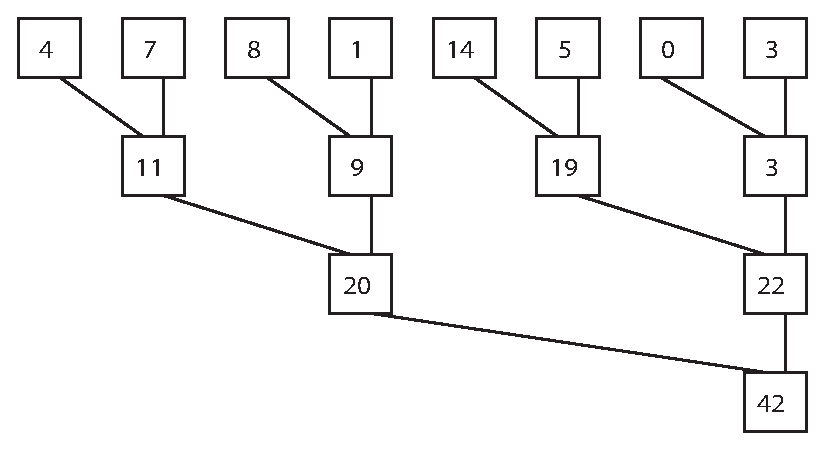
\includegraphics{parallel-left-fold-tree.pdf}
\caption{An illustration of the successive reduction of
  parallel-left-fold where $\oplus$ is set to be addition.}
\end{figure}
\vspace{1pc}

This figure is drawn with parent nodes right aligned to indicate that
the result of the addition ends up overwriting the slot originally
occupied by the second summand. The bottom-most value in each column
of the graphical representation will be the final value stored in the
temporary array that stores intermediate sums.

An explicit procedure to determine which processor performs each
$\oplus$ operation must be devised to complete this implementation of
parallel-left-fold. Note that each level in this tree represents a reduction of the original input
sequence. Since we have a balanced binary tree, the number of nodes at
the $j$th level (starting at 0) of the tree is  $\lceil \frac{n}{2^j}
\rceil$. Thus we need $\lceil \frac{n}{2^i}\rceil$ processors to
perform the $i$th (starting at 1) reduction of our sequence.
Note that there are exactly $\lceil \frac{p}{2^j} \rceil = \lceil
\frac{n}{2^{j+1}} \rceil$ numbers $l$ in the range 0 to $p-1$ for
which $(l \mod 2^j = 0)$. This means that the modulus operator can be
used, together with a variable that is multiplied by two in each
iteration to select which processors will be active. Since all $p$ of
our processors must be active in the first round, we will initialize
this variable to the value of 1. Note that this value also corresponds
to the distance between the values that each processor will add in any
particular reduction. The following pseudo-code describes the rest of
the details of the implementation.

\begin{algorithm}[h!]
\caption{parallel-left-fold where $p = n/2$ and $n=2^k$}
\begin{algorithmic}
\STATE values[pid] $\leftarrow$ input[$2\cdot \mbox{pid}$] $\oplus$ input[$2\cdot \mbox{pid} +1$]
\STATE stride $\leftarrow$ 1
\WHILE{$\mbox{pid} \mod \frac{n}{\mbox{stride}} = 0$ and $\mbox{stride} < n$}
\STATE values[pid] $\leftarrow$ values[pid] $\oplus$ values[pid $+$ stride] 
\STATE stride $\leftarrow$ stride$\cdot 2$
\ENDWHILE
\RETURN values[0]
\end{algorithmic}
\end{algorithm}

%%Since each of the computations a particular depth in the tree above are computed in lock step, the height of the tree is the running time of parallel-left fold.  Since the tree above is a balanced binary tree with $n$ leaves it has height $\lceil log_2 n \rceil$. This result can also be obtained by solving the recurrence relation (\ref{rr}) with the base case $T(1) = 0$.%%

\vspace{3pc}
\subsection{A First Attempt}

In computing parallel-left-fold in the manner described above, some of the partial sums that constitute the output of parallel-prefix-sums are computed.

\begin{figure}[h]
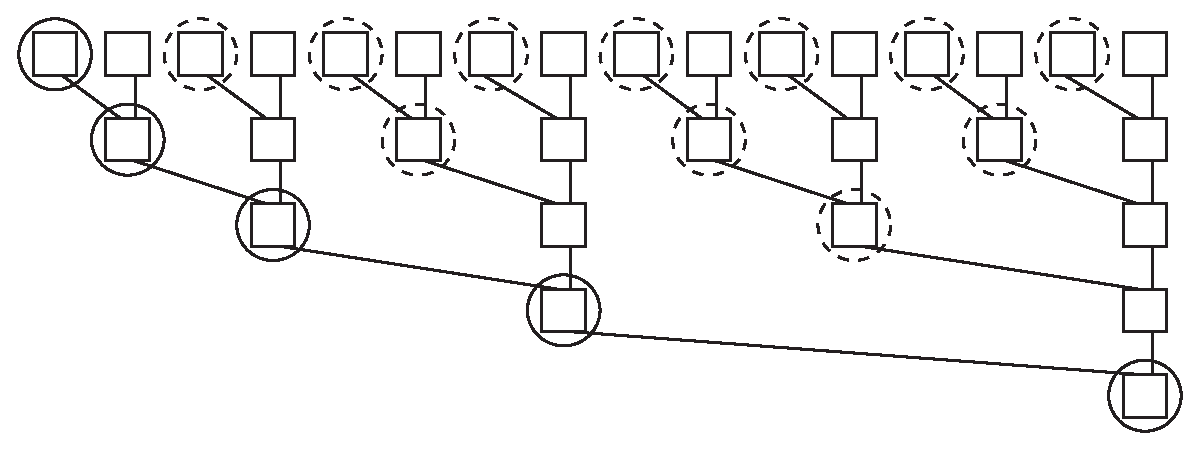
\includegraphics[scale = .75]{correctsums.pdf}
\caption{Each node in the tree that represents the final value in a slot of the temporary array is circled. A solid line indicates that the value is correct, while a dashed line indicates that the value is incorrect.}
\end{figure}
\vspace{1pc}

Specifically, all the partial sums that are placed at output indices
$2^a-1$ for positive integers $a$ are correct. The other sums that are
computed as intermediaries to the final sum are incomplete in the
sense that they are only correct prefix sums for some continuous
subsequence of the input sequence.

In general, the sum in the temporary array at the $i$th index after
the execution of parallel-left fold is the sum of the subsequence
ending at $a_i$, and including $2^j$ terms\footnote{$a_{i-(2^j-1)},
  a_{i-(2^j-1)+1}, \ldots a_i$}, where $j$ is the final round in which
that value was modified.

\begin{proof}
What we will prove is that the value at any array index $i$ that is active during the $j$th reduction is the subsequence of length $2^j$ ending at the $i$th value of the input sequence. This directly implies that the value that remains after the execution of the entire algorithm will be the value after the final reduction in which that value was changed.

We prove this claim by induction on $j$. When $j=0$ the values in the temporary array are just the values of the input sequence. Since $j=0$, $2^j = 1$, and indeed, the values of the input sequence are the trivial sums of length one, 

Suppose that the node $i$  is active during the $j+1$th reduction step. Then by our induction assumption, its value just before that reduction step is executed is the correct subsequence of length $2^j$. Similarly, the array value that is to be added to our value was also active at the $j$th reduction

\footnote{The value at the $z$th array index is active in the $j+1$th
  round when $z+1 \mod 2^{j+1} = 0$ (and $z \neq 0$). Thus $z - 2^j +
  1 = 0 \mod 2^j$, since both $z+1$ and $2^j = 0 \mod 2^j$. This is
  the index of the value on the left hand side of the $\oplus$
  operation.}

, and so its subsequence is the $\oplus$ of the sequence of length
$2^j$ ending at that index. As noted in the previous section, the
distance between terms added in the $j$th reduction is always $2^j$,
which means that these two sequences have no overlapping terms, and no
missing terms in between them. By the associativity of the operator
that is being used, the value that results from applying $\oplus$ to
these two terms is value of the subsequence ending at the rightmost index of length $2^j + 2^j = 2 \cdot 2^j = 2^{j+1}$.
\end{proof}

With this fact in hand, it is easy to determine which array indices
contain correct values. Since the value at the $i$th index of the
array is correct when it contains the $\oplus$ of the $i$ terms, any
index $i$ for which $i+1 = \max \{ 2^a : i+1 \mod 2^a = 0 \}$ will contain
a correct value. It is easy to see that this condition is only
satisfied when $i+1 = 2^a$ for some $a$.

\begin{algorithm}[h!]
\caption{parallel-prefix-sums where $p = n/2$ and $n=2^k$}
\begin{algorithmic}
\STATE output[pid] $\leftarrow$ input[$2\cdot \mbox{pid}$] $\oplus$
\STATE stride $\leftarrow$ 1
\WHILE{$\mbox{pid} \mod \frac{n}{\mbox{stride}} = 0$ and $\mbox{stride} < n$}
\STATE values[pid] $\leftarrow$ values[pid] $\oplus$ values[pid $+$ stride] 
\STATE stride $\leftarrow$ stride$\cdot 2$
\ENDWHILE
\RETURN

\STATE myitem $\leftarrow$ pid $\cdot 2$ 
\STATE segmentsize $= n/2$
\WHILE{stride $> 0$}
\IF{myitem $\mod$ segmentsize $= 0$ and pid $!=$ 0}
\STATE values[myitem -1 + segmentsize/2] += values[myitem-1]
\ENDIF
\STATE segmentsize = segmentsize/2

\ENDWHILE
\end{algorithmic}
\end{algorithm}
	
\chapter*{Conclusion}
         \addcontentsline{toc}{chapter}{Conclusion}
	\chaptermark{Conclusion}
	\markboth{Conclusion}{Conclusion}
	\setcounter{chapter}{4}
	\setcounter{section}{0}
	

    \appendix
      \chapter{The First Appendix}



  \backmatter 

    \bibliographystyle{bsts/mla-good} % there are a variety of styles available; 
    \nocite{*}
    \bibliography{thesis}
\end{document}
